\documentclass[a4paper]{article}

%%%%%%%%%%%%%%%%%%%%%%%%%%%%%%%%%%%%%%%%%%%%%%%%%%%%%%%%%%%%%%%%%%%%%%%%%%%%%%%

\usepackage[utf8]{inputenc}
\usepackage[T1]{fontenc}
\usepackage[english]{babel}
\usepackage{caption}
\usepackage{subcaption}
\usepackage{float}
\usepackage{hyperref}
\usepackage{fancyhdr}
\usepackage[a4paper, left=2.85cm, right=2.85cm]{geometry}
\usepackage{graphicx}
\usepackage[nottoc]{tocbibind}
\usepackage[bottom]{footmisc}
\graphicspath{{images/}}

\pagestyle{fancy}
\fancyhf{}
\rhead{\small Paris-Saclay University -- 23/11/2021}
\lhead{\small Gaëtan Serré -- Master AI}
\rfoot{\thepage}

\begin{document}

\setlength{\parindent}{0pt}

\newgeometry{
  bottom=1.5cm
}
\setlength{\headheight}{13.59999pt}
\addtolength{\topmargin}{-1.59999pt}

\begin{center}
  \vspace*{5cm}

  \textbf{\large Performing Regression on Complex Data using a
  Squeeze-and-Excitation Residual Neural Network, Chess as a Model System}

  \vspace*{1cm}

  Gaëtan Serré \\
  {\ttfamily gaetan.serre@universite-paris-saclay.fr}

  \vspace*{10cm}

  \vfill
  \noindent\rule{\textwidth}{0.4pt}
  \begin{figure}[H]
      \centering
      \begin{subfigure}{.35\textwidth}
          
\includegraphics[width=\textwidth]{ups-logo.png}
      \end{subfigure}
  \end{figure}
\end{center}
\pagenumbering{gobble}

\pagebreak
\restoregeometry
\pagebreak
\pagenumbering{arabic}

\begin{abstract}
\noindent
As neural networks for image recognition become more and more powerful
and AI becomes more and more present in all fields,
it would be very helpful to be able to use these models
with non-image data and get good performance.
This paper aims to show that this is possible through an model system very
related to artificial intelligence: chess.

\noindent
We can simplify a chess engine in two main components: an evaluation function,
which is a function that takes a chess position as input and returns a score 
(usually, $>0$ if Whites are winning and $<0$ if Blacks are winning) and
a search algorithm which will uses the evaluation function to find the best move
to play in a given position. Generally, we ask the search algorithm to search
at a certain depth $d$ meaning that our engine will return the best move to play
by searching $d$ moves in advance.

\noindent
I introduce GAiA, a chess engine which uses a Squeeze-and-Excitation\cite{squeezeandexcitation}
residual network as an evaluation function and the Stockfish\cite{stockfish} 
search algorithm which is known for its efficiency. GAiA's neural network
try to reproduce the evaluation function of Stockfish 14.
With only few hours of training, GAiA's neural network has
an accuracy of 0.92 (using the coefficient of determination).

\noindent
These results suggest that Squeeze-and-Excitation residual networks,
which are the state-of-the-art neural networks for image recognition,
can be used with data that are not images.
\end{abstract}

\section{Introduction}
Artificial intelligence for image recognition is becoming
increasingly powerful. Since 2015, thanks to the ResNet\cite{resnet}
architecture, We achieve astounding performance on the ImageNet database.
Furthermore, in 2017 is introduced Squeeze-and-Excitation\cite{squeezeandexcitation}
network architecture which significantly
improve the performance of ResNet with almost no computation costs.

The question is: can we use this architecture on data that are not
originally images. If so, we just have to encode our data in 3-dimensional
tensors and look for the number of Squeeze-and-Excitation residual
blocks (Figure \ref{fig:seblock}) that optimizes our results to get excellent performance.
The challenge is to know if Squeeze-and-Excitation networks are
generalizable to any kind of machine learning problem.

As a chess fan, I have chosen to show that it was possible to create a
high-performance chess engine using this type of neural network.
I have called this chess engine GAiA.

\begin{figure}[H]
  \centering
  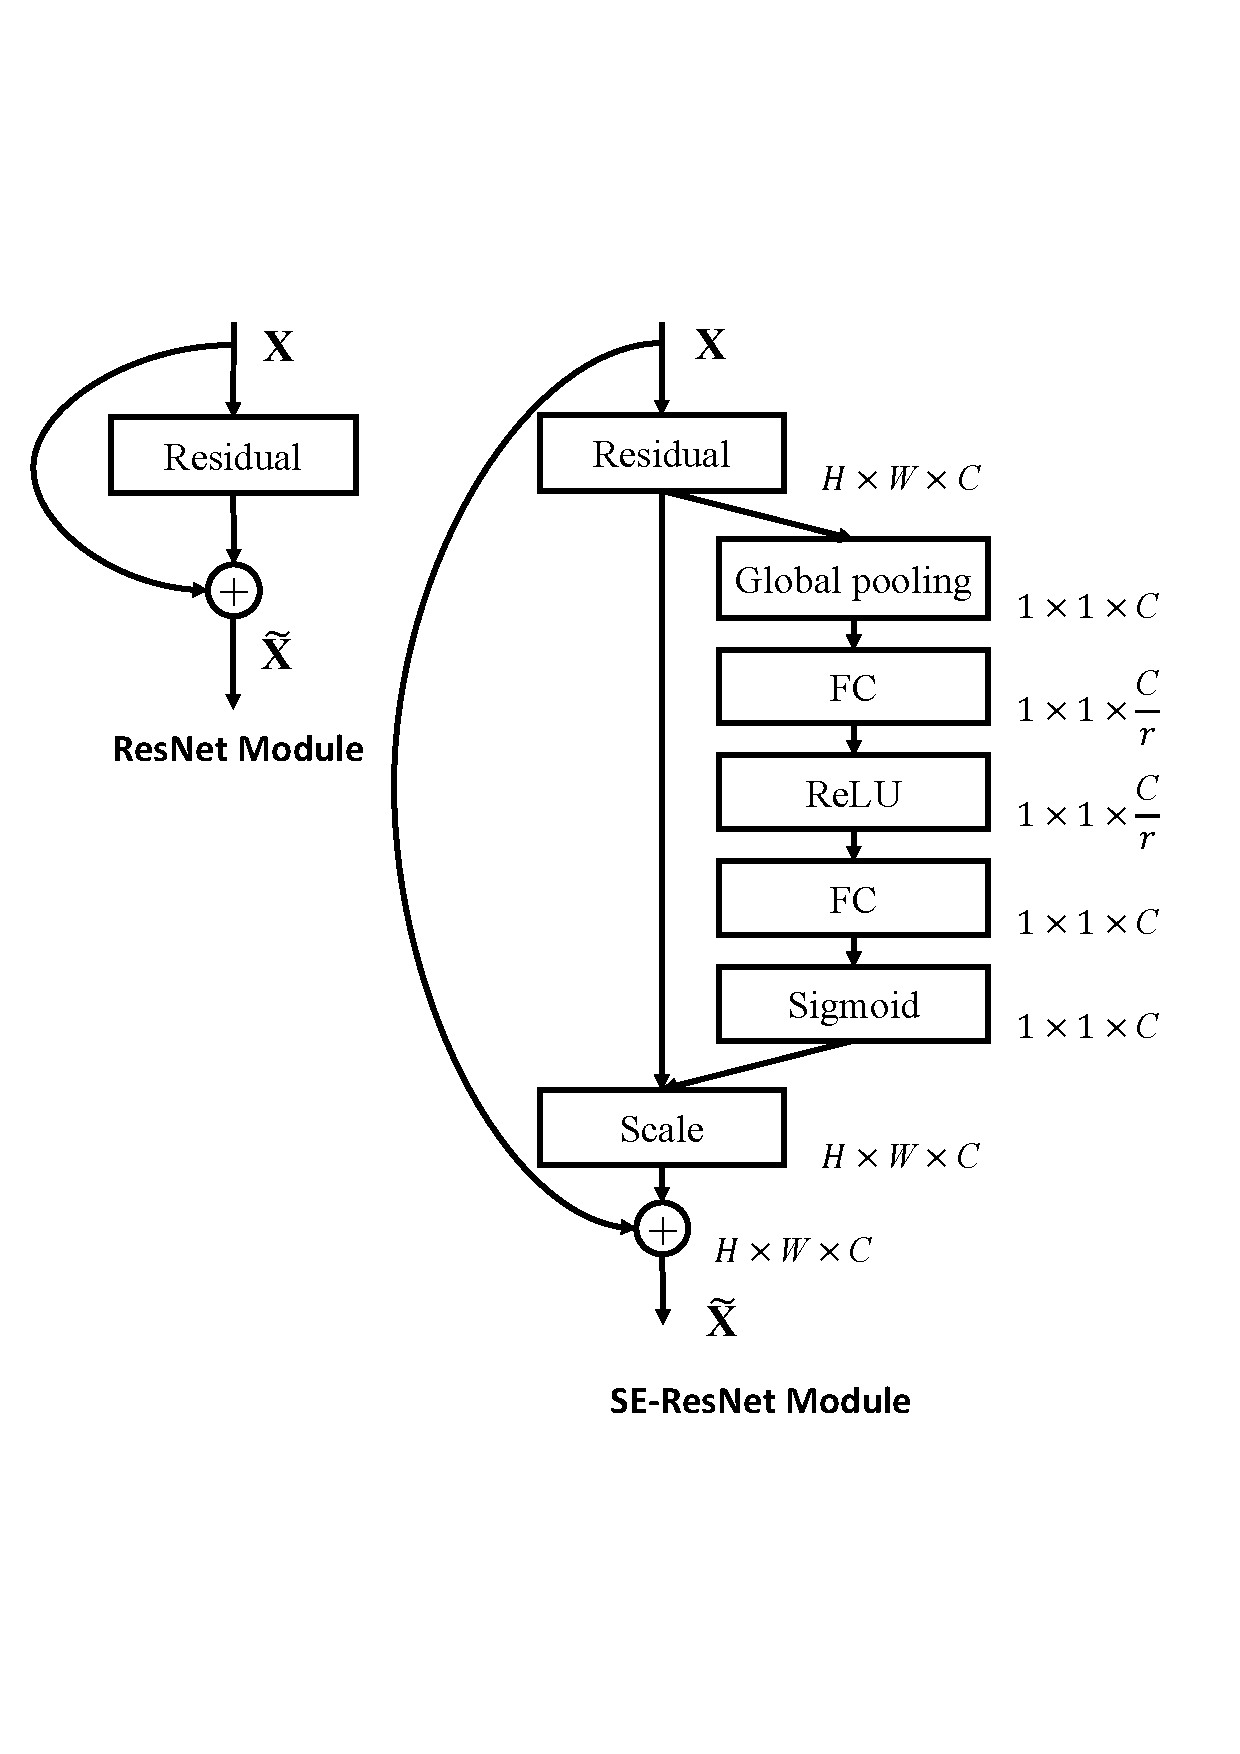
\includegraphics[width=8cm]{module_seresnet.pdf}
  \caption{The schema of the original Residual block (left) and the SE-ResNet
  block (right)}
  \label{fig:seblock}
\end{figure}

\section{Data}
GAiA's neural network tries to recreate the evaluation function of Stockfish 14,
a open-source world reknown chess engine. It uses heuristics function written
by human experts to evaluate position. Stockfish also uses a classical
alpha-beta game tree search with plenty optimizations to find the best move.
GAiA is a combination of the Stockfish game tree search algorithm and a
Squeeze-and-Excitation residual neural network as evaluation function.

In order to train GAiA's neural network, I needed tons of different
chess position. Lichess.org\cite{lichess} is a popular, free and open-source
chess platform which provides millions of games played by humans every month.
From these games, I extracted millions of different positions along with their
Stockfish 14 evaluation.
Each position is encoded as a $8\times8$ image with $15$ channels: 
$12$ representing each chess pieces, $1$ for the actual player, $1$
for the en-passant square and $1$ for the castling rights.

\section{Neural Network Structure}
My model architecture is composed of $3$ SE-ResNet blocks of $2$ CNNs with $64$ filters
and a kernel shape of $1\times1$ using ReLU activation function. The output is a
fully connected layer with a linear readout function(Figure \ref{fig:model_archi}).
This model architecture is designed based on Maia\cite{maia}.
The loss is the Mean Absolute Error and the accuracy the coefficient of determination.
I used the framework Tensorflow 2.7 to create and train the neural network.
I tried several numbers of SE-ResNet blocks and $3$ seemed
to be the best compromise between computing costs and results
(Figure \ref{fig:acc_loss} \& \ref{fig:score_valid}).
The model is trained on $\sim 400k$ positions and tested on $\sim 150k$ during 30 epochs (Figure \ref{fig:history}).

\begin{figure}[htp]
  \centering
  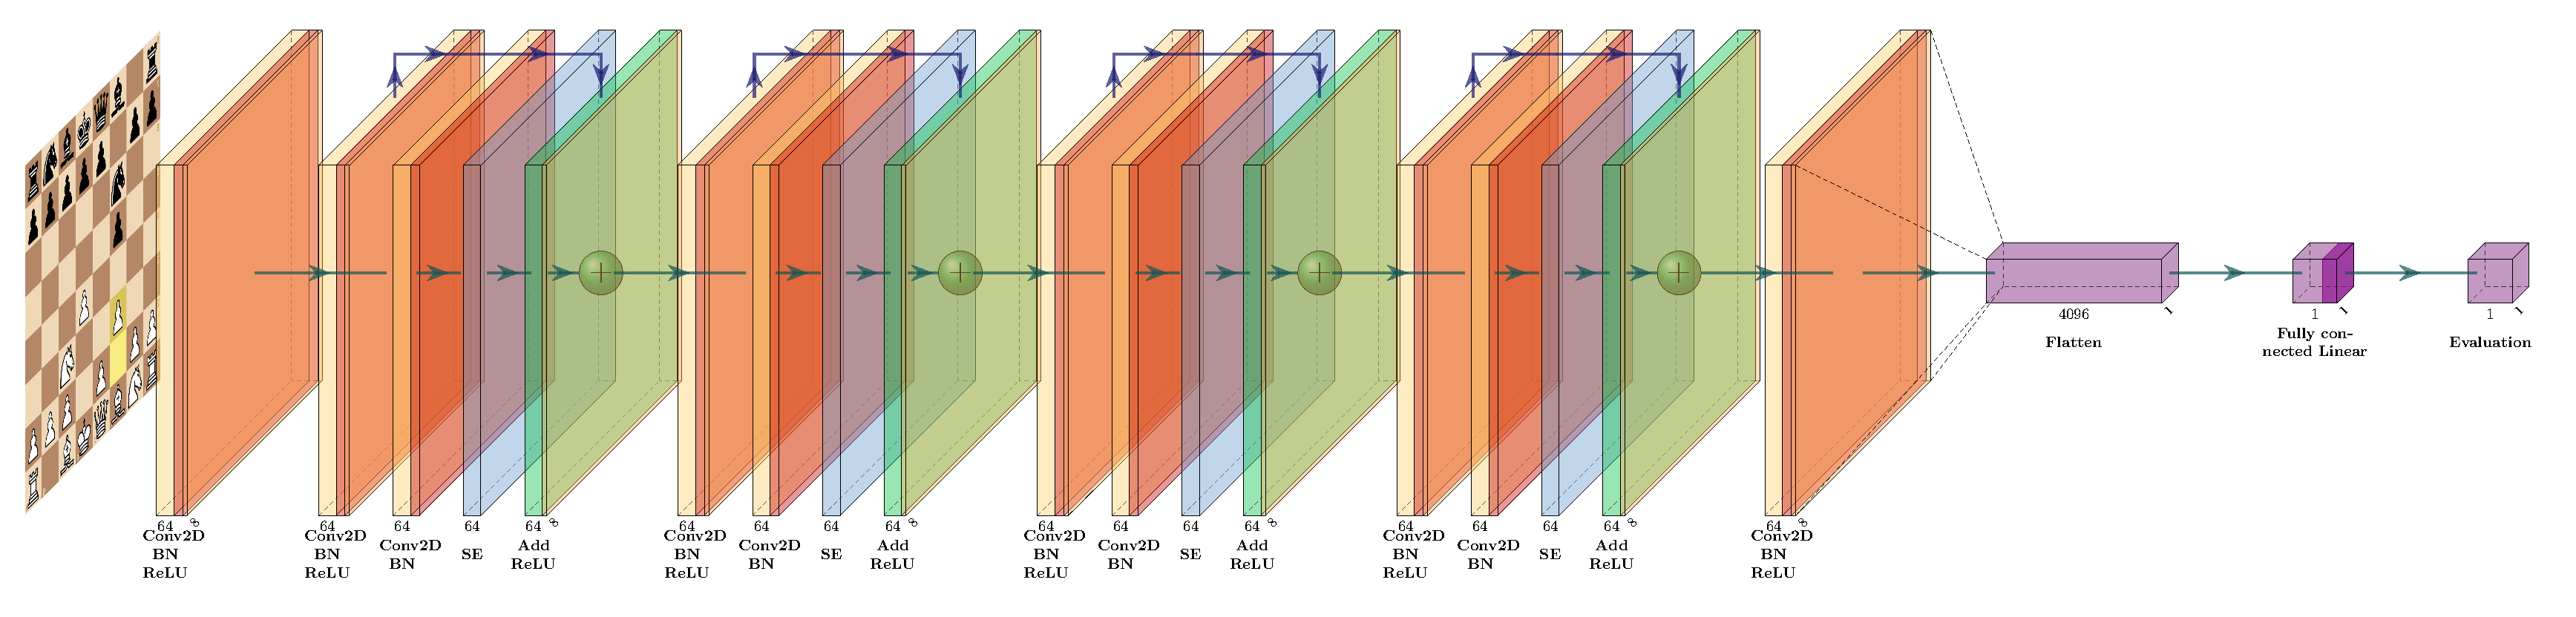
\includegraphics[width=13cm]{network/network.pdf}
  \caption{GAiA's neural network architecture}
  \label{fig:model_archi}
\end{figure}

\begin{figure}[H]
  \centering
  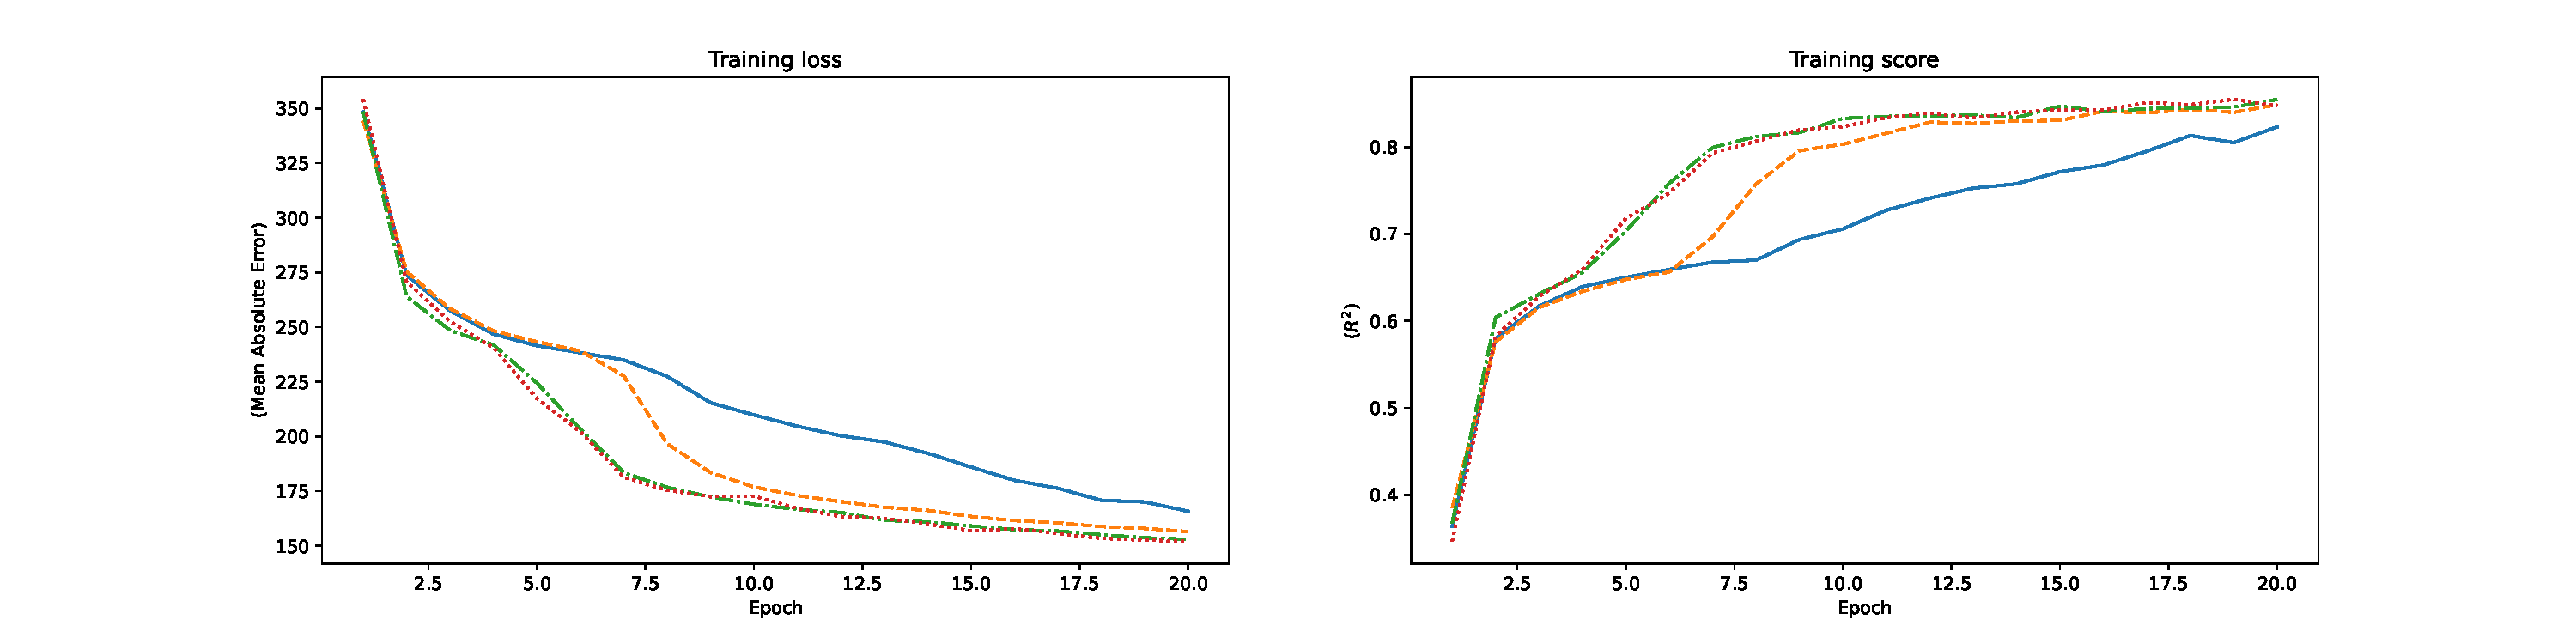
\includegraphics[width=15cm]{model_selection_1.pdf}
  \caption{Loss and accuracy on train sets}
  \label{fig:acc_loss}
\end{figure}

\begin{figure}[H]
  \centering
  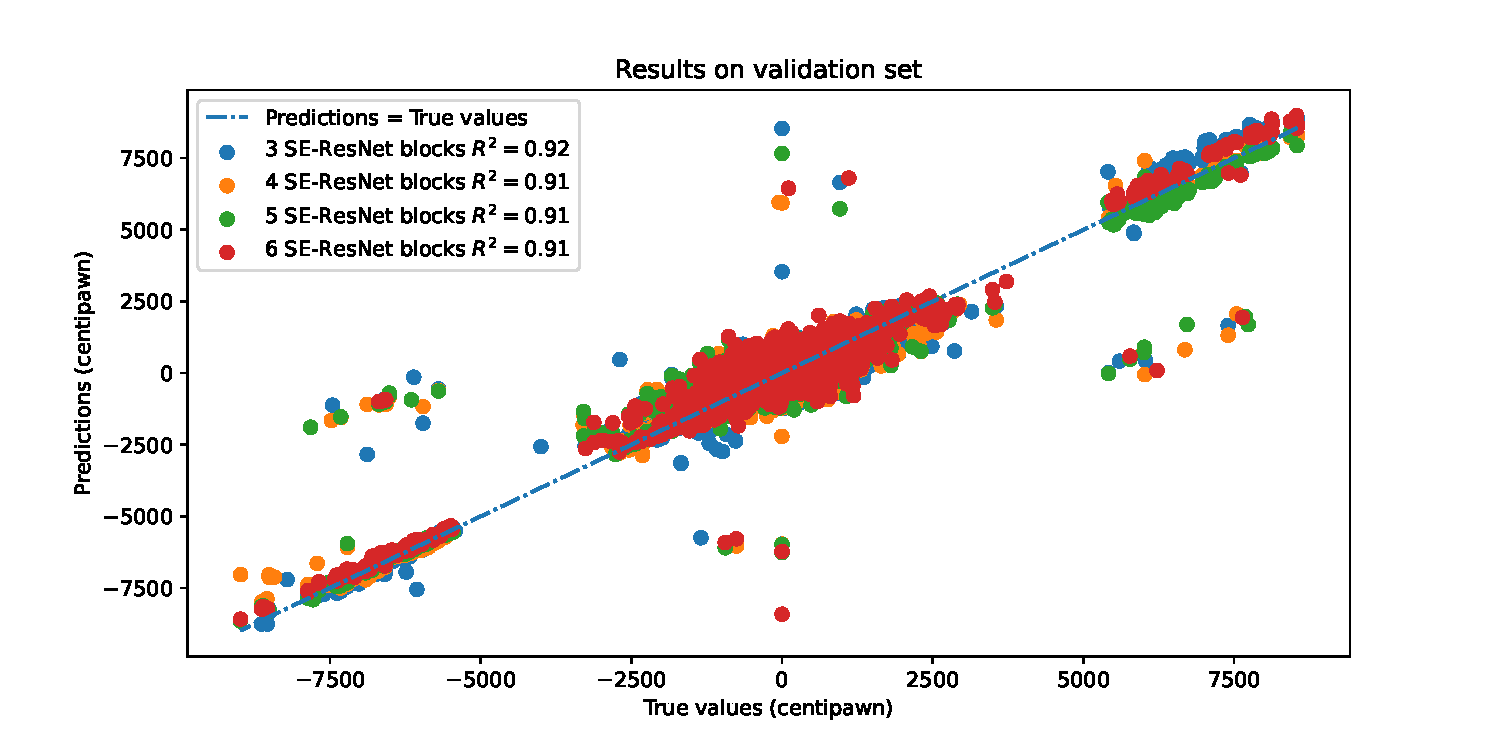
\includegraphics[width=13cm]{model_selection_2.pdf}
  \caption{Score on validation sets}
  \label{fig:score_valid}
\end{figure}

\begin{figure}[H]
  \centering
  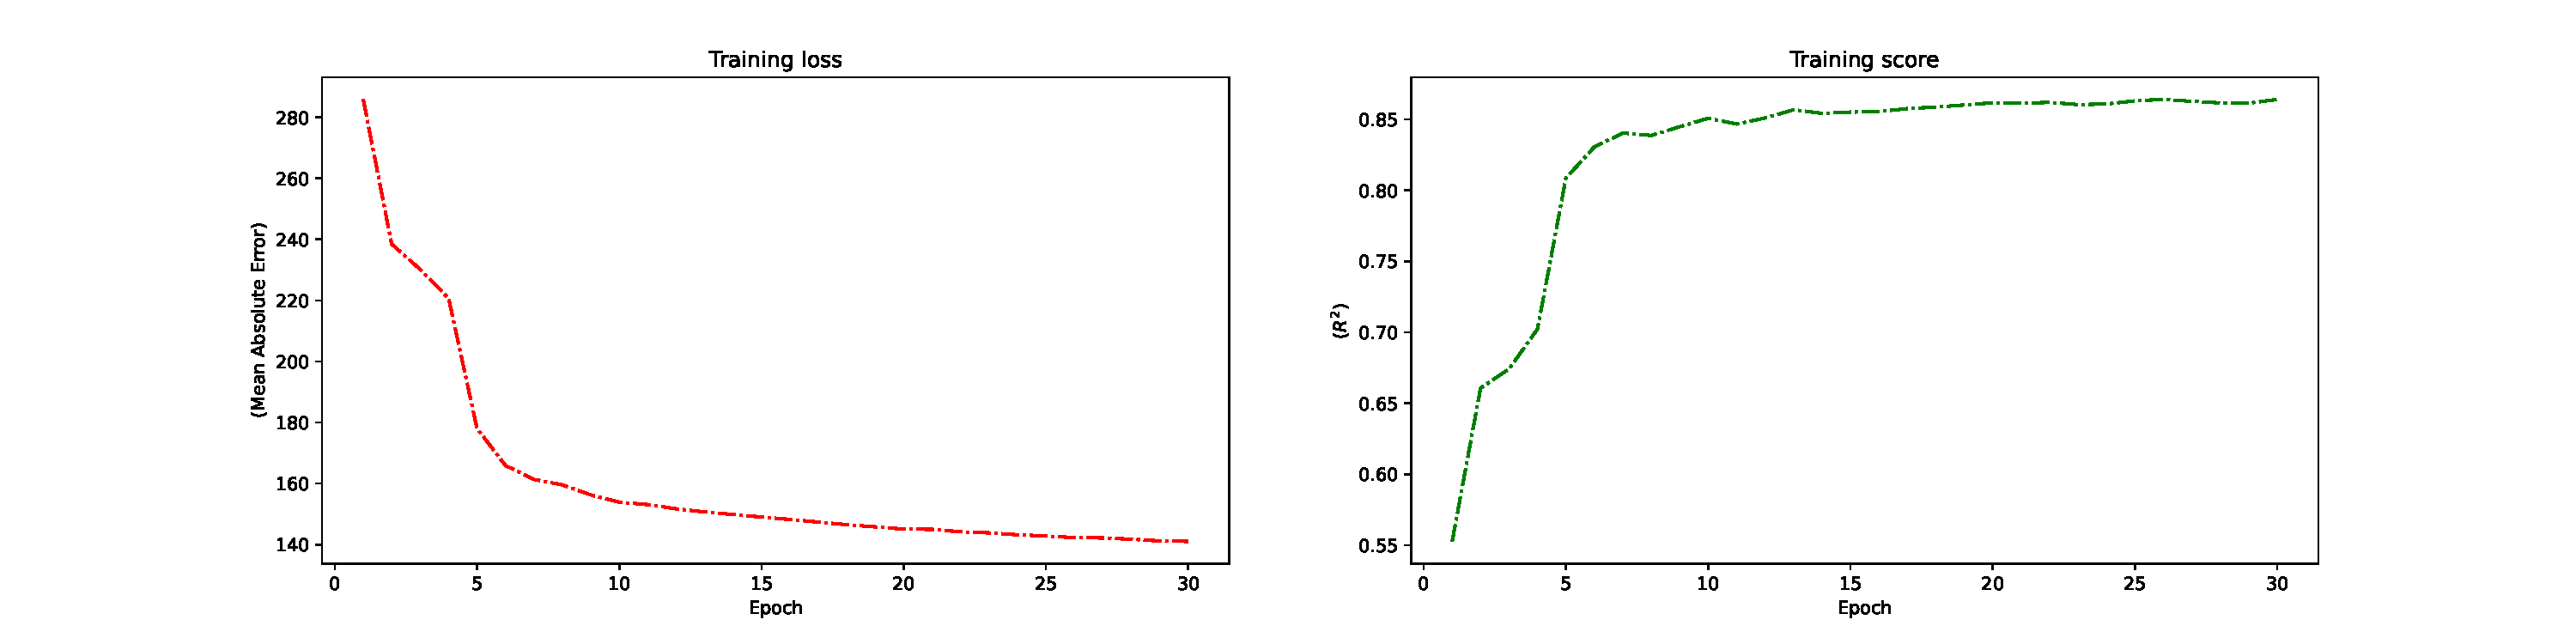
\includegraphics[width=15cm]{GAiA_history.pdf}
  \caption{Loss and accuracy during training}
  \label{fig:history}
\end{figure}

\section{Results}
As we can see in the figure \ref{fig:result}, GAiA's neural network
has great performance and I only trained it on $\sim 400k$ positions.
Moreover, GAiA (the complete chess engine) works pretty well:
since infer a board evaluation through a such complex neural network
is much more time consuming than use heuristics functions, GAiA can see
much less positions per second than standard chess engine. However,
it has been able to defeat many engines on Lichess.org around 2000 elo.


\begin{figure}[H]
  \centering
  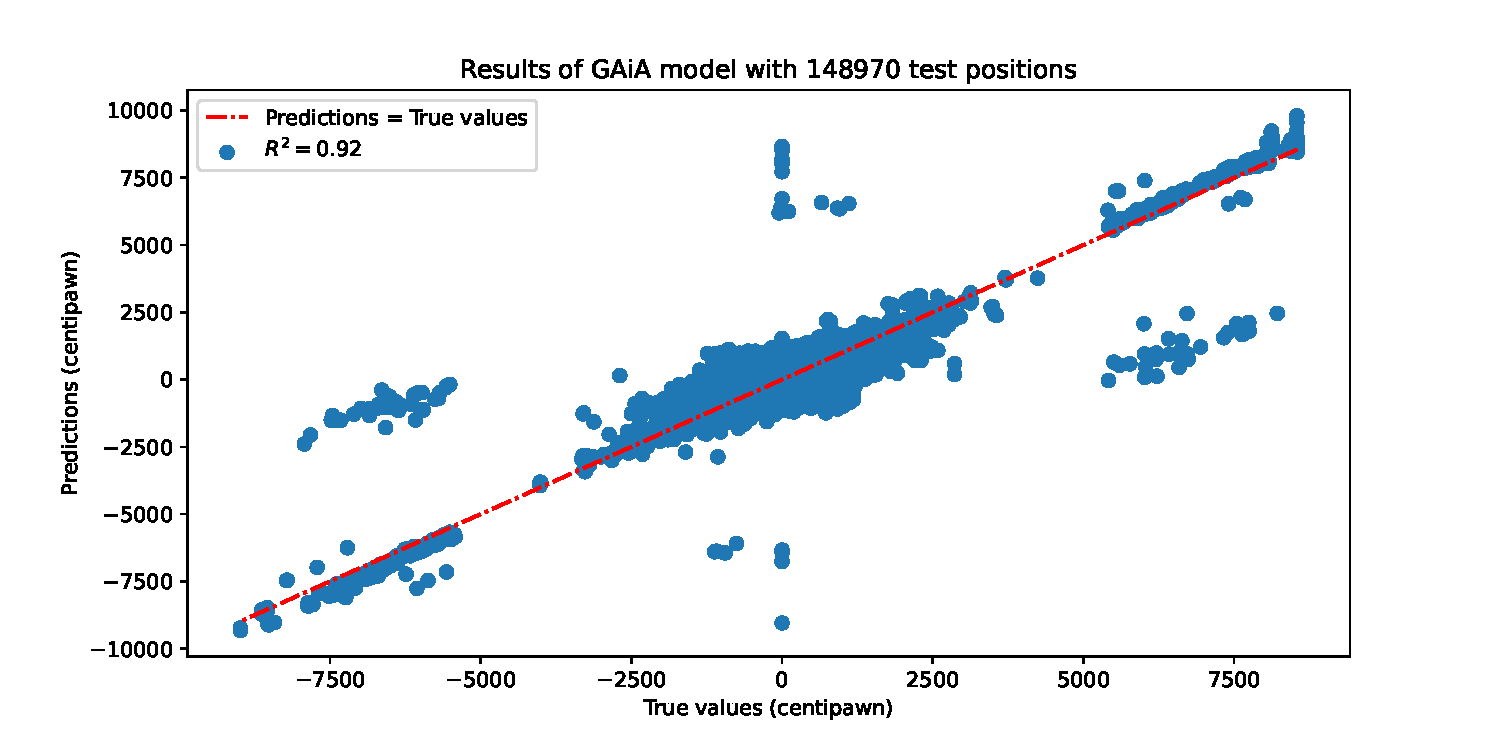
\includegraphics[width=13cm]{result.pdf}
  \caption{GAiA's neural network results}
  \label{fig:result}
\end{figure}

\section{Conclusion}
Artificial intelligence is being used in more and more fields.
It is becoming very complex to design models capable of answering very precise problems.
We could see through this article that it was possible (for some problems) to transform
our data into images in order to use a neural network specialized in image recognition.
It may not be the most efficient model but it allows to have very good performances easily.
In my chess example, I was able to design a chess engine able to beat any non-professional
human player in only a few hours of training. It would be interesting to find other problems
that can be solved in this way to corroborate these results.

\bibliographystyle{abbrv}
\bibliography{refs}


\end{document}